\begin{figure}[htbp]
\centering
\shorthandoff{<>}
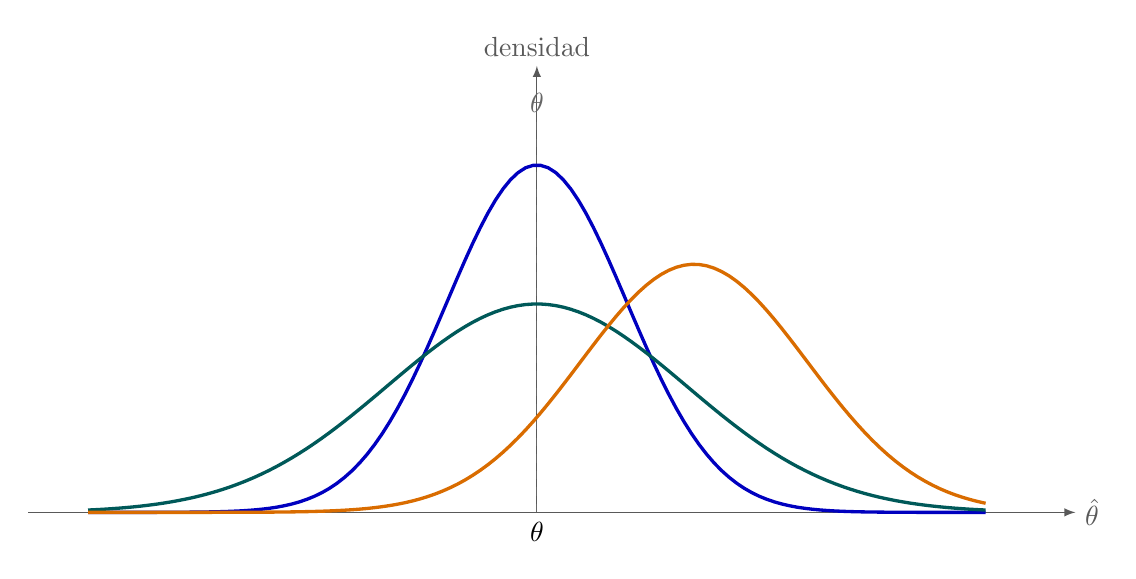
\begin{tikzpicture}[x=1.9cm,y=4.2cm,font=\normalsize,>=latex]
  \draw[->,black!65] (-3.4,0) -- (3.6,0) node[right] {$\hat\theta$};
  \draw[->,black!65] (0,0) -- (0,1.35) node[above] {densidad};
  \draw[dashed,black!60] (0,0) -- (0,1.18) node[above] {$\theta$};
  \draw[blue!75!black,very thick,domain=-3:3,samples=120]
    plot (\x,{1.05*exp(-\x*\x/0.72)});
  \draw[teal!70!black,very thick,domain=-3:3,samples=120]
    plot (\x,{0.63*exp(-\x*\x/2.0)});
  \draw[orange!85!black,very thick,domain=-3:3,samples=120]
    plot (\x,{0.75*exp(-((\x-1.05)*(\x-1.05))/1.15)});
  \node[below] at (0,0) {$\theta$};
\end{tikzpicture}
\shorthandon{<>}
\caption{Esquema conceptual de distribuciones muestrales de estimadores. La curva azul concentra más probabilidad cerca de $\theta$; la verde está centrada en $\theta$ pero es más dispersa; la naranja está desplazada. Es una ilustración de sesgo y precisión, no un conjunto de datos del problema.}
\label{fig:estimadores}
\end{figure}